\documentclass[border=2pt]{standalone}

\usepackage{fontspec}
    \setmainfont{Times New Roman}
\usepackage[dvipsnames]{xcolor}
    \definecolor{GDLcolor}{HTML}{d0cece}
    \definecolor{ELcolor}{HTML}{f3f1c5}
    \definecolor{LDLcolor}{HTML}{c5eaf9}
\usepackage{tikz}
\usetikzlibrary{%
    calc,
    math,
    decorations.pathreplacing, % 画括号的
    decorations.pathmorphing
}
\usepackage{amsmath}

\begin{document}
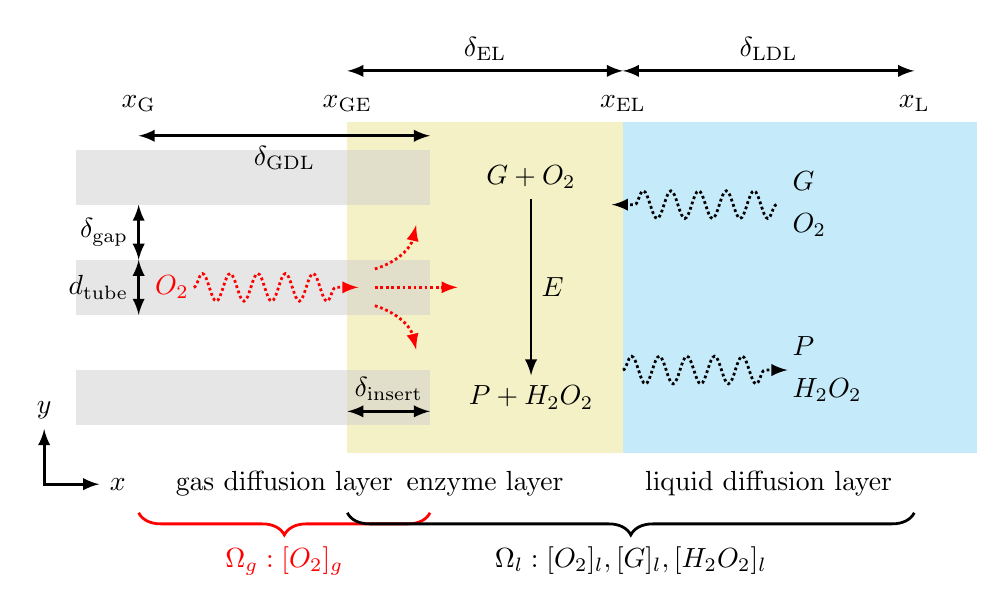
\begin{tikzpicture}[line width=1pt]
    \tikzmath{%
        \deltasnake=1.95;
        \offset=0.8;
        % 纳米管
        \deltatube=4.5;
        \dtube=0.7;
        \numtube=3;
        \numgap=\numtube;
        \epsilonGDL=0.5;
        \deltagap=((1-\epsilonGDL)/\epsilonGDL)*\dtube;
        % 气体扩散层、酶层和液体扩散层
        \deltaGDL=\deltatube-\offset;
        \deltaEL=3.5;
        \deltaLDL=\deltatube-\offset;
        \deltafig=\numtube*\dtube+\numgap*\deltagap;
        % 进气管插入酶层的比例
        \phiinsert=0.3;
        \deltainsert=\phiinsert*\deltaEL;
    };

    \coordinate (O) at (0, 0); % 原点,就定xG界面为原点吧
    % \fill [red] (O) circle (2pt);
    \coordinate (xG) at ($ (O) + (0, \deltafig) $);
    \coordinate (xGE) at ($ (O) + (\deltaGDL-\deltainsert, \deltafig) $);
    \coordinate (xEL) at ($ (O) + (\deltaGDL-\deltainsert+\deltaEL, \deltafig) $);
    \coordinate (xL) at ($ (O) + (\deltaGDL-\deltainsert+\deltaEL+\deltaLDL, \deltafig) $);
    \coordinate (GDL) at ($ (O) + (\deltaGDL/2, -0.1) $);
    \coordinate (EL) at ($ (O) + (\deltaGDL-\deltainsert+\deltaEL/2, -0.1) $);
    \coordinate (LDL) at ($ (O) + (\deltaGDL-\deltainsert+\deltaEL+\deltaLDL/2, -0.1) $);

    % axes
    \draw [-latex, line cap=rect] ($ (O) + (-1.2, -0.4) $) -- ++(0.7, 0) node [right] {$ x $};
    \draw [-latex, line cap=rect] ($ (O) + (-1.2, -0.4) $) -- ++(0, 0.7) node [above] {$ y $};

    % 酶层
    \fill [ELcolor] (\deltaGDL-\deltainsert, 0) rectangle ++(\deltaEL, \deltafig);
    % 液体扩散层
    \fill [LDLcolor] (\deltaGDL-\deltainsert+\deltaEL, 0) rectangle ++(\deltaLDL+\offset, \deltafig);
    % 纳米管
    \foreach \i in {0, ..., 2} {%
            \fill [GDLcolor, fill opacity=0.5] ($ (O) + (-\offset, {\i*(\deltagap+\dtube)+\deltagap/2}) $) rectangle ++(\deltatube, \dtube);
        }

    % 顶部node
    \node (xG) [above] at (xG) {$ x_{\mathrm{G}} $};
    \node (xGE) [above] at (xGE) {$ x_{\mathrm{GE}} $};
    \node (xEL) [above] at (xEL) {$ x_{\mathrm{EL}} $};
    \node (xL) [above] at (xL) {$ x_{\mathrm{L}} $};
    \draw [latex-latex] ($ (O) + (0, \deltafig-1/4*\deltagap) $) -- (\deltaGDL, \deltafig-1/4*\deltagap)
    node (deltaGDL) [midway, below] {$ \delta_{\mathrm{GDL}} $};
    % \draw [latex-latex] ([yshift=3pt] xG.north) -- ([yshift=3pt] xGE.north)
    % node (deltaGDL) [midway, above] {$ \delta_{\mathrm{GDL}} $};
    \draw [latex-latex] ([yshift=5pt] xGE.north) -- ([yshift=5pt] xEL.north)
    node (deltaEL) [midway, above] {$ \delta_{\mathrm{EL}} $};
    \draw [latex-latex] ([yshift=5pt] xEL.north) -- ([yshift=5pt] xL.north)
    node (deltaLDL) [midway, above] {$ \delta_{\mathrm{LDL}} $};

    \draw [latex-latex] ($ (O) + (0, \dtube+3/2*\deltagap) $) -- ++(0, \dtube) node [midway, left] {$ d_{\mathrm{tube}} $};
    \draw [latex-latex] ($ (O) + (0, 2*\dtube+3/2*\deltagap) $) -- ++(0, \deltagap) node [midway, left] {$ \delta_{\mathrm{gap}} $};
    % \draw [latex-latex] ($ (O) + (-\offset, \deltagap/4) $) -- ++(\deltatube, 0) node [midway, below] {$ \delta_\mathrm{tube} $};
    \draw [latex-latex] ($ (O) + (\deltaGDL-\deltainsert, {\deltagap/2+1/4*\dtube}) $) -- ++(\deltainsert, 0) node [midway, above] {$ \delta_\mathrm{insert} $};

    % 底部node
    \node [below] at (GDL) {gas diffusion layer};
    \node [below] at (EL) {enzyme layer};
    \node [below] at (LDL) {liquid diffusion layer};
    \draw [red, decorate, decoration={brace, mirror, amplitude=8pt}] ($ (xG) + (0, -\deltafig-1) $) -- ($ (xGE) + (\deltainsert, -\deltafig-1) $)
    node [midway, below=0.3cm] {$ \Omega_g: [O_2]_g $};
    \draw [decorate, decoration={brace, mirror, amplitude=8pt}] ($ (xGE) + (0, -\deltafig-1) $) -- ($ (xL) + (0, -\deltafig-1) $)
    node [midway, below=0.3cm] {$ \Omega_l: [O_2]_l, [G]_l, [H_2 O_2]_l $};

    % 中间node
    %% O_2 diffusion into EL
    \draw [dash pattern=on 1pt off 1pt, color=red, decorate, decoration={snake, amplitude=5pt}] ($ (O) + ({\deltaGDL-\deltainsert-\deltasnake}, \deltafig/2) $) node [left=-2pt] {$ O_2 $} -- ++(\deltasnake, 0);
    \draw [-latex, color=red] ($ (O) + ({\deltaGDL-\deltainsert}, \deltafig/2) $) -- ++(4pt, 0);
    \draw [-latex, color=red, dash pattern=on 1pt off 1pt] ($ (O) + ({\deltaGDL-\deltainsert+1/3*\deltainsert}, \deltafig/2+1/3*\dtube) $) to [bend right] ++(\deltainsert/2, 4/5*\dtube);
    \draw [-latex, color=red, dash pattern=on 1pt off 1pt] ($ (O) + ({\deltaGDL-\deltainsert+1/3*\deltainsert}, \deltafig/2-1/3*\dtube) $) to [bend left] ++(\deltainsert/2, -4/5*\dtube);
    \draw [-latex, color=red, dash pattern=on 1pt off 1pt] ($ (O) + ({\deltaGDL-\deltainsert+1/3*\deltainsert}, \deltafig/2) $) -- ++(\deltainsert, 0);
    %% G, O_2 diffusion into EL
    \draw [dash pattern=on 1pt off 1pt, color=black, decorate, decoration={snake, amplitude=5pt}] ($ (O) + ({\deltaGDL+\deltaEL-\deltainsert+\deltasnake}, 3/4*\deltafig) $)
    node [right=2pt] {
        $
            \begin{aligned}
                 & G   \\
                 & O_2
            \end{aligned}
        $
    } -- ++(-\deltasnake, 0);
    \draw [-latex] ($ (O) + ({\deltaGDL+\deltaEL-\deltainsert}, 3/4*\deltafig) $) -- ++(-4pt, 0);
    %% P, H2O_2 out of EL
    \draw [dash pattern=on 1pt off 1pt, color=black, decorate, decoration={snake, amplitude=5pt}] ($ (O) + ({\deltaGDL+\deltaEL-\deltainsert}, 1/4*\deltafig) $) -- ++(\deltasnake, 0)
    node [right=2pt] {
        $
            \begin{aligned}
                 & P       \\
                 & H_2 O_2
            \end{aligned}
        $
    };
    \draw [-latex] ($ (O) + ({\deltaGDL+\deltaEL+\deltasnake-\deltainsert}, 1/4*\deltafig) $) -- ++(4pt, 0);
    %% G + O_2 -> P + H_2 O_2
    \node (reactants) at ($ (O) + ({\deltaGDL+2/3*\deltaEL-\deltainsert}, 5/6*\deltafig) $) {$ G + O_2 $};
    \node (products) at ($ (O) + ({\deltaGDL+2/3*\deltaEL-\deltainsert}, 1/6*\deltafig) $) {$ P + H_2 O_2 $};
    \draw [-latex] (reactants) -- (products) node [midway, right] {$ E $};
\end{tikzpicture}
\end{document}
